%% Submissions for peer-review must enable line-numbering
%% using the lineno option in the \documentclass command.
%%
%% Preprints and camera-ready submissions do not need
%% line numbers, and should have this option removed.
%%
%% Please note that the line numbering option requires
%% version 1.1 or newer of the wlpeerj.cls file.

\documentclass[fleqn,10pt,numbers]{wlpeerj} % for journal submissions
% \documentclass[fleqn,10pt]{wlpeerj} % for preprint submissions

\usepackage{lmodern}
\usepackage[T1]{fontenc}
\usepackage[utf8]{inputenc}
\usepackage[scaled=0.8]{DejaVuSansMono}

\usepackage{graphicx}
\usepackage[all]{xy}
\usepackage{amsmath}
\usepackage{caption}
\graphicspath{ {images/} }

% Makes quote characters in monospace font not be curly
\usepackage{upquote}

\usepackage{amsmath}
\usepackage{url}

% Order matters here
\usepackage{xr-hyper}
\usepackage{hyperref}
\externaldocument[S-]{supplement}

\hypersetup{
  colorlinks=true,
  urlcolor=blue,
  citecolor=black,
  filecolor=black % cross-file links, which do not actually work unless the
                  % supplement is named supplement.pdf
}

% for nice units
\usepackage{siunitx}

% for images: png, pdf, etc
\usepackage{graphicx}

% for nice table formatting, i.e., /toprule, /midrule, etc
\usepackage{booktabs}

% to allow for \verb++ declarations in captions.
\usepackage{cprotect}

% to allow usage of \mathbb symbols
\usepackage{amssymb}

\usepackage{longtable}

\usepackage{listings}

\newcommand\email[1]{\href{mailto:#1}{#1}}
\title{SymPy: symbolic computing in Python}

\input{authors}

% \keywords{Python, computer algebra system, symbolics}

\begin{abstract}
  SymPy is an open source computer algebra system written in pure Python. It
  is built with a focus on extensibility and ease of use, through both
  interactive and programmatic applications. These characteristics have led
  SymPy to become a popular symbolic library for the scientific Python
  ecosystem. This paper presents the architecture of SymPy, a description of
  its features, and a discussion of select submodules. The
  supplementary material provide additional examples and further outline
  details of the architecture and features of SymPy.
\end{abstract}

\begin{document}

\flushbottom
\maketitle
\thispagestyle{empty}

\section{Introduction}

%% What sympy is, where to download etc.
%%
%% List other major CAS's.
%%
%% Why SymPy.

SymPy is a full featured computer algebra system (CAS) written in the
Python~\cite{lutz2013learning}
programming language.
It is free and open source software, licensed under the 3-clause BSD
license~\cite{rosen2005open}.
The SymPy project was started by Ond\v{r}ej \v{C}ert\'{\i}k in 2005, and it has
since grown to over 500 contributors. Currently, SymPy is
developed on GitHub using a bazaar community
model~\cite{raymond1999cathedral}. The accessibility of the codebase and the
open community model allow SymPy to rapidly respond to the needs of
users and developers.

Python is a dynamically typed programming language that has a focus on
ease of use and readability.\footnote{\label{note:python}This paper assumes a moderate
  familiarity with the Python programming language.} Due in part to this focus, it has become a popular
language for scientific
computing and data science, with a broad ecosystem of
libraries~\cite{oliphant2007python}. SymPy is itself used as a dependency
by many libraries
and tools to support research within a variety of domains, such as
SageMath~\cite{sagemath} (pure and applied mathematics),
yt~\cite{2011ApJS..192....9T} (astronomy and astrophysics),
PyDy~\cite{gede2013constrained} (multibody dynamics), and
SfePy~\cite{cimrman2014sfepy} (finite elements).

Unlike many CAS's, SymPy does not invent its own programming language. Python
itself is used both for the internal implementation and end user
interaction. By using the operator overloading functionality of Python, SymPy follows the embedded domain specific language paradigm proposed by Hudak~\cite{dsl-little-languages}.  The exclusive usage of a single programming language makes it easier
for people already familiar with that language to use or develop SymPy.
Simultaneously, it enables developers to focus on mathematics, rather than
language design.  SymPy version 1.0 officially supports Python 2.6, 2.7 and 3.2--3.5.

SymPy is designed with a strong focus on usability as a library.
Extensibility is important in its application program interface
(API) design. Thus, SymPy makes no attempt to extend
the Python language itself. The goal is for users of SymPy to be able to
include SymPy alongside other Python libraries in their workflow, whether that
be in an interactive environment or as a programmatic part in a larger system.

Being a library, SymPy does not have a built-in graphical user interface (GUI).
However, SymPy exposes a rich interactive display system, and supports
registering display formatters with Jupyter~\cite{kluyver2016jupyter} frontends,
including the Notebook and Qt Console, which will render SymPy expressions
using MathJax~\cite{cervone2012mathjax} or \LaTeX{}.

The remainder of this paper discusses key components of the SymPy library.
Section~\ref{sec:features} enumerates the features of SymPy and takes a closer
look at some of the important ones. The section~\ref{sec:numerics} looks at
the numerical features of SymPy and its dependency library, mpmath.
Section~\ref{sec:domain_specific} looks at the domain specific physics
submodules for performing symbolic and numerical calculations in classical
mechanics and quantum mechanics. Section~\ref{sec:architecture} discusses the
architecture of SymPy. Section~\ref{sec:other-proj} looks at a selection of
packages that depend on SymPy. Conclusions and future directions for SymPy are given
in section~\ref{sec:conclusion}. All examples in this paper use SymPy version
1.0 and mpmath version 0.19.

Additionally, the supplementary material takes a deeper look at a few SymPy
topics. Supplement section~\ref{S-suppsec:Gruntz} discusses the Gruntz
algorithm, which SymPy uses to calculate symbolic limits.
Sections~\ref{S-suppsec:Series}--\ref{S-suppsec:numsimpl} of the supplement
discuss the series, logic, Diophantine equations, sets, statistics, category
theory, tensor, and numerical simplification submodules of SymPy,
respectively. Supplement section~\ref{S-suppsec:examples} provides additional
examples for topics discussed in the main paper. Supplement
section~\ref{S-suppsec:sympy-gamma} discusses the SymPy Gamma project.
Finally, section~\ref{S-suppsec:comp-mma} of the supplement contains a brief
comparison of SymPy with Wolfram Mathematica.

The following statement imports all SymPy functions into the global Python
namespace.\footnote{\texttt{import *} has been used here to aid the
  readability of the paper, but is best to avoid such wildcard import
  statements in production code, as they make it unclear which names are
  present in the namespace. Furthermore, imported names could clash with
  already existing imports from another package. For example, SymPy, the
  standard Python \texttt{math} library, and NumPy all define the \texttt{exp}
  function, but only the SymPy one will work with SymPy symbolic expressions.}
From here on, all examples in this paper assume that this statement has been
executed:\footnote{\label{note:prompt} The three greater-than signs denote the user input for the
  Python interactive session, with the result, if there is one, shown on the
  next line.}

\begin{verbatim}
>>> from sympy import *
\end{verbatim}

All the examples in this paper can be tested on
\href{http://live.sympy.org}{SymPy Live}, an online Python shell that uses the
Google App Engine~\cite{ciurana2009developing} to execute SymPy code. SymPy Live
is also integrated into the SymPy documentation at
\href{http://docs.sympy.org}{http://docs.sympy.org}.


\section{Overview of Capabilities}
\label{sec:features}

%% List of Features and how to use
%%
%% Quick overview of the main modules, what it can do and so on. It should probably provide examples how to use sympy.
%%
%% See also the supplement (below)

% Features to discuss in depth:
This section gives a basic introduction of SymPy, and lists its features.
A few features---assumptions, simplification, calculus, polynomials, printers,
solvers, and matrices---are core components of SymPy and are discussed in
depth. Many other features are discussed in depth in the supplementary
material.

\subsection{Basic Usage}
\label{sec:basic-usage}
% symbols, various ways to declare them

Symbolic variables, called symbols, must be defined and assigned to
Python variables before they can be used. This is typically done through the
\texttt{symbols} function, which may create multiple symbols in a single
function call. For instance,
\begin{verbatim}
>>> x, y, z = symbols('x y z')
\end{verbatim}
creates three symbols representing variables named $x$, $y$, and $z$. In this
particular instance, these symbols are all assigned to Python variables of the
same name. However, the user is free to assign them to different
Python variables, while representing the same symbol, such as
\texttt{a, b, c = symbols(\textquotesingle{}x y z\textquotesingle{})}.
In order to minimize potential confusion, though, all examples in this paper will
assume that
the symbols \verb|x|, \verb|y|, and \verb|z| have been assigned to Python variables
identical to their symbolic names.

Expressions are created from symbols using Python's mathematical syntax.  For
instance, the following Python code creates the expression $(x^2 - 2x + 3)/y$.
Note that the expression remains unevaluated: it is represented symbolically.

\begin{verbatim}
>>> (x**2 - 2*x + 3)/y
(x**2 - 2*x + 3)/y
\end{verbatim}


\subsection{List of Features}

Although SymPy's extensive feature set cannot be covered in depth in this
paper, bedrock areas, that is, those areas that are used throughout the
library, are discussed in their own
subsections below. Additionally, Table~\ref{features-table} gives a compact listing
of all major capabilities present in the SymPy codebase. This grants a
sampling from the breadth of topics and application domains that SymPy
services. Unless stated otherwise, all features noted in
Table~\ref{features-table} are symbolic in nature. Numeric features are
discussed in Section~\ref{sec:numerics}.

\begin{longtable}[htbc]{>{\raggedright}p{0.30\linewidth}p{0.63\linewidth}}
\caption{SymPy Features and Descriptions.\label{features-table}}\\
\toprule
\textbf{Feature (submodules)} & \textbf{Description} \\
\midrule
Calculus (\texttt{sympy.core}, \texttt{sympy.calculus}, \texttt{sympy.integrals}, \texttt{sympy.series}) & Algorithms for computing derivatives, integrals, and limits.\\

Category Theory (\texttt{sympy.categories}) & Representation of objects, morphisms, and diagrams. Tools
for drawing diagrams with Xy-pic~\cite{rose1999xy}.\\

Code Generation (\texttt{sympy.printing}, \texttt{sympy.codegen}) & Generation of compilable and executable code in a
variety of different programming languages from expressions directly. Target
languages include C, Fortran, Julia, JavaScript,
Mathematica, MATLAB and Octave, Python, and Theano.\\

Combinatorics \& Group Theory (\texttt{sympy.combinatorics}) & Permutations, combinations,
partitions, subsets, various permutation groups (such as polyhedral, Rubik,
symmetric, and others), Gray codes~\cite{Nijenhuis1978combinatorial},
and Prufer sequences~\cite{biggs1976graph}.\\

Concrete Math (\texttt{sympy.concrete}) & Summation, products, tools for determining whether summation
and product expressions are convergent, absolutely convergent, hypergeometric,
and for determining other properties; computation of Gosper's normal form~\cite{Petkovsek1997AeqB} for two univariate polynomials.\\

Cryptography (\texttt{sympy.crypto}) & Block and stream ciphers, including shift, Affine,
substitution, Vigen\`{e}re's, Hill's, bifid, RSA, Kid RSA,
linear-feedback shift registers, and Elgamal encryption.\\

Differential Geometry (\texttt{sympy.diffgeom}) & Representations of manifolds, metrics, tensor
products, and coordinate systems in Riemannian and pseudo-Riemannian
geometries~\cite{sussman2013functional}.\\
% TODO: Someone verify that this is a good summary of the diffgeom module

Geometry (\texttt{sympy.geometry}) & Representations of 2D geometrical entities, such as lines and
circles. Enables queries on these entities, such as asking the area of an
ellipse, checking for collinearity of a set of
points, or finding the intersection between objects.\\

Lie Algebras (\texttt{sympy.liealgebras}) & Representations of Lie algebras and root systems.\\

Logic (\texttt{sympy.logic}) & Boolean expressions, equivalence testing, satisfiability, and normal
forms.\\

Matrices (\texttt{sympy.matrices}) & Tools for creating matrices of symbols and expressions.
Both sparse and dense representations, as well as symbolic linear
algebraic operations (e.g., inversion and factorization), are
supported.\\

Matrix Expressions (\texttt{sympy.matrices.expressions}) & Matrices with symbolic dimensions (unspecified entries).
Block matrices.\\

Number Theory (\texttt{sympy.ntheory}) & Prime number generation, primality testing, integer
factorization, continued fractions, Egyptian fractions, modular arithmetic,
quadratic residues, partitions, binomial and multinomial coefficients,
prime number tools, hexidecimal digits of $\pi$, and integer factorization. \\

Plotting (\texttt{sympy.plotting}) & Hooks for visualizing expressions via matplotlib~\cite{Hunter:2007}
or as text drawings when lacking a graphical back-end. 2D function plotting,
3D function
plotting, and 2D implicit function plotting are supported.\\

Polynomials (\texttt{sympy.polys}) & Polynomial algebras over various coefficient domains.
Functionality ranges from simple operations (e.g., polynomial division) to
advanced computations (e.g., Gr\"obner bases~\cite{Adams1994intro} and multivariate
factorization over algebraic number domains).\\

Printing (\texttt{sympy.printing}) & Functions for printing SymPy expressions in the terminal with ASCII
or Unicode characters and converting SymPy expressions to \LaTeX{} and
MathML.\\

Quantum Mechanics (\texttt{sympy.physics.quantum}) & Quantum states, bra--ket notation, operators, basis sets,
representations, tensor products, inner products, outer products, commutators,
anticommutators, and specific quantum system implementations.\\

Series (\texttt{sympy.series}) & Series expansion, sequences, and limits of sequences.
This includes Taylor, Laurent, and Puiseux series as well as special series, such
as Fourier and formal power series.\\

Sets (\texttt{sympy.sets}) & Representations of empty, finite, and infinite sets (including
special sets such as the natural, integer, and complex numbers). Operations
on sets such as union, intersection, Cartesian product, and building sets from
other sets are supported.\\

Simplification (\texttt{sympy.simplify}) & Functions for manipulating and simplifying expressions.
Includes algorithms for simplifying hypergeometric functions, trigonometric
expressions, rational functions, combinatorial functions, square root
denesting, and common subexpression elimination.\\

Solvers (\texttt{sympy.solvers}) & Functions for symbolically solving equations, systems
of equations, both linear and non-linear, inequalities, ordinary differential
equations, partial differential equations, Diophantine equations, and
recurrence relations.\\

Special Functions (\texttt{sympy.functions}) & Implementations of a number of well known special functions,
including Dirac delta, Gamma, Beta, Gauss error functions, Fresnel integrals,
Exponential integrals, Logarithmic integrals, Trigonometric integrals, Bessel,
Hankel, Airy, B-spline, Riemann Zeta, Dirichlet eta, polylogarithm, Lerch
transcendent, hypergeometric, elliptic integrals, Mathieu, Jacobi polynomials,
Gegenbauer polynomial, Chebyshev polynomial, Legendre polynomial, Hermite
polynomial, Laguerre polynomial, and
spherical harmonic functions.\\

Statistics (\texttt{sympy.stats}) & Support for a random variable type as well as the ability to
declare this variable from prebuilt distribution functions such as
Normal, Exponential, Coin, Die, and other custom distributions~\cite{rocklin2012symbolic}.\\

Tensors (\texttt{sympy.tensor}) & Symbolic manipulation of indexed objects.\\

Vectors (\texttt{sympy.vector}) & Basic operations on vectors and differential calculus with respect
to 3D Cartesian coordinate systems.\\
\bottomrule

\end{longtable}

%% Assumptions
\subsection{Assumptions}
\label{sec:assumptions}
The assumptions system allows users to specify that symbols have certain
common mathematical properties, such as being positive, imaginary, or
integer. SymPy is careful to never perform simplifications on an expression
unless the assumptions allow them. For instance, the simplification $\sqrt{t^2}
= t$ holds if $t$ is nonnegative ($t\ge 0$), but it does not hold for a general
complex $t$.%
\footnote{In SymPy, $\sqrt{z}$ is defined on the usual principal branch with
the branch cut along the negative real axis.}


By default, SymPy performs all calculations assuming that symbols are
complex valued. This assumption makes it easier to treat mathematical problems
in full generality.
\begin{verbatim}
>>> t = Symbol('t')
>>> sqrt(t**2)
sqrt(t**2)
\end{verbatim}

By assuming the most general case, that \texttt{t} is complex by default, SymPy
avoids performing mathematically invalid operations. However, in many cases
users will wish to simplify expressions containing terms like $\sqrt{t^2}$.

Assumptions are set on \texttt{Symbol} objects when they are created. For
instance \texttt{Symbol(\textquotesingle{}t\textquotesingle{}, positive=True)} will create a symbol named
\texttt{t} that is assumed to be positive.
\begin{verbatim}
>>> t = Symbol('t', positive=True)
>>> sqrt(t**2)
t
\end{verbatim}

Some of the common assumptions are
\texttt{negative}, \texttt{real}, \texttt{nonpositive}, \texttt{integer},
\texttt{prime} and \texttt{commutative}.\footnote{SymPy assumes that two
  expressions $A$ and $B$ commute with each other multiplicatively, that is,
  $A\cdot B=B\cdot A$, unless they both have \texttt{commutative=False}. Many
  algorithms in SymPy require special consideration to work correctly with
  noncommutative products.} Assumptions on any SymPy object can be checked with the
\verb|is_|\texttt{\textit{assumption}} attributes, like \verb|t.is_positive|.

Assumptions are only needed to restrict a domain so that certain
simplifications can be performed. They are not required to make the domain match
the input of a function. For instance, one can create the object
$\sum_{n=0}^m f(n)$ as \verb|Sum(f(n), (n, 0, m))| without setting
\texttt{integer=True} when creating the Symbol object \texttt{n}.

The assumptions system additionally has deductive capabilities. The
assumptions use a three-valued logic using the Python built in objects
\texttt{True}, \texttt{False}, and \texttt{None}. Note that \texttt{False}
is returned if the SymPy object doesn't or can't have the assumption.
For example, both \texttt{I.is\_real} and \texttt{I.is\_prime} return
\texttt{False} for the imaginary unit \texttt{I}.

\texttt{None} represents the ``unknown'' case. This could mean that given
assumptions do not unambiguously specify the truth of an attribute. For
instance, \texttt{Symbol(\textquotesingle{}x\textquotesingle{},
  real=True).is\_positive} will give \texttt{None} because a real symbol might
be positive or negative. \texttt{None} could also mean that not enough is
known or implemented to compute the given fact. For instance, \texttt{(pi +
  E).is\_irrational} gives \texttt{None}---indeed, the rationality of
$\pi + e$ is an open problem in mathematics~\cite{lang1966introduction}.

Basic implications between the facts are used to deduce assumptions.
Deductions are made using the Rete
algorithm~\cite{doorenbos1995production}.\footnote{\label{note:assumptions}For
  historical reasons, this algorithm is distinct from the \texttt{sympy.logic}
  submodule, which is discussed in section~\ref{S-suppsec:Logic} of the
  supplementary material. SymPy also has an experimental assumptions system
  which stores facts separate from objects, and uses \texttt{sympy.logic} and
  a SAT solver for deduction. We will not discuss this system here.} For
instance, the assumptions system knows that being an integer implies being
rational.
\begin{verbatim}
>>> i = Symbol('i', integer=True)
>>> i.is_rational
True
\end{verbatim}
Furthermore, expressions compute the assumptions on themselves
based on the assumptions of their arguments. For instance, if \texttt{x} and
\texttt{y} are both created with \texttt{positive=True}, then
\texttt{(x + y).is\_positive} will be \texttt{True} (whereas
\texttt{(x - y).is\_positive} will be \texttt{None}).


\subsection{Simplification}

% polynomial expressions

% functions

% expand( ), factor( ), collect( ), together( ), apart( )
%% maybe a table best suits this part.

% simplification: simplify, sqrt denest, fu, trigsimp

The generic way to simplify an expression is by calling the \texttt{simplify}
function.
It must be emphasized that simplification is not a rigorously defined
mathematical operation~\cite{Moses1971simplification}.
The \texttt{simplify} function applies several simplification routines along
with heuristics to make the output expression ``simple''.\footnote{The
\texttt{measure} parameter of the \texttt{simplify}
function lets the user specify the Python function used to determine how complex an
expression is.  The default measure function returns the total number of
operations in the expression.}

It is often preferable to apply more directed simplification functions. These
apply very specific rules to the input expression and are typically able to make
guarantees about the output. For instance, the \texttt{factor} function,
given a polynomial with rational coefficients in several variables,
is guaranteed to
produce a factorization into irreducible factors. Table~\ref{simplify-table}
lists common simplification functions.

Examples for these simplification functions can be found in
section~\ref{S-suppsec:examples} of the supplementary material.

\begin{center}
\begin{table}[htb]
\caption{Some SymPy Simplification Functions}\label{simplify-table}
\begin{tabular}{ll}
\toprule
\verb|expand| & expand the expression \\
\verb|factor| & factor a polynomial into irreducibles \\
\verb|collect| & collect polynomial coefficients \\
\verb|cancel| & rewrite a rational function as $p/q$ with common factors
canceled \\
\verb|apart| & compute the partial fraction decomposition of a rational function
\\
\verb|trigsimp| & simplify trigonometric expressions~\cite{fu2006automated} \\
\verb|hyperexpand| & expand hypergeometric functions~\cite{Roach1996hyper,roach1997meijerg} \\
\bottomrule
\end{tabular}
\end{table}
\end{center}


\subsection{Calculus}
\label{sec:calculus}
SymPy provides all the basic operations of calculus, such as calculating
limits, derivatives, integrals, or summations.

Limits are computed with the \verb|limit| function, using the Gruntz
algorithm~\cite{Gruntz1996limits} for computing symbolic limits and heuristics
(a description of the Gruntz algorithm may be found in
section~\ref{S-suppsec:Gruntz} of the supplementary material).
For example, the following computes
$\lim\limits_{x\to \infty} x\sin(\frac{1}{x})=1$. Note that SymPy denotes
$\infty$ as \verb|oo| (two lower case ``\verb|o|''s).
\begin{verbatim}
>>> limit(x*sin(1/x), x, oo)
1
\end{verbatim}
As a more complex example, SymPy computes \[\lim\limits_{x\to 0}{\left(2 e^{\frac{1 - \cos{\left (x \right )}}{\sin{\left (x \right )}}} -
  1\right)}^{\frac{\sinh{\left (x \right )}}{\operatorname{atan}^{2}{\left (x
      \right )}}} = e.\]
\begin{verbatim}
>>> limit((2*exp((1-cos(x))/sin(x))-1)**(sinh(x)/atan(x)**2), x, 0)
E
\end{verbatim}

Derivatives are computed with the \verb|diff| function, which recursively uses
the various differentiation rules.
\begin{verbatim}
>>> diff(sin(x)*exp(x), x)
exp(x)*sin(x) + exp(x)*cos(x)
\end{verbatim}

Integrals are calculated with the \verb|integrate| function. SymPy
implements a combination of the Risch
algorithm~\cite{bronstein2005integration}, table lookups, a reimplementation
of Manuel Bronstein's ``Poor Man's Integrator''~\cite{Bronstein2005pmint}, and
an algorithm for computing integrals based on Meijer G-functions~\cite{Roach1996hyper,roach1997meijerg}. These allow
SymPy to compute a wide variety of indefinite and definite integrals. The
Meijer G-function algorithm and the Risch algorithm are respectively
demonstrated below by the computation of \[\int_{0}^{\infty} e^{-s t}\log{\left (t \right )}\, dt = - \frac{ \log{\left (s \right )} + \gamma}{s}\] and \[\int \frac{- 2 x^{2} \left(\log{\left (x \right )} + 1\right) e^{x^{2}} + {\left(e^{x^{2}} + 1\right)}^{2}}{x {\left(e^{x^{2}} + 1\right)}^{2} \left(\log{\left (x \right )} + 1\right)}\, dx = \log{\left (\log{\left (x \right )} + 1 \right )} + \frac{1}{e^{x^{2}} + 1}.\]
\begin{verbatim}
>>> s, t = symbols('s t', positive=True)
>>> integrate(exp(-s*t)*log(t), (t, 0, oo)).simplify()
-(log(s) + EulerGamma)/s
>>> integrate((-2*x**2*(log(x) + 1)*exp(x**2) +
... (exp(x**2) + 1)**2)/(x*(exp(x**2) + 1)**2*(log(x) + 1)), x)
log(log(x) + 1) + 1/(exp(x**2) + 1)
\end{verbatim}

Summations are computed with the \verb|summation| function, which uses a
combination of Gosper's algorithm~\cite{gosper1978decision}, an algorithm that
uses Meijer G-functions~\cite{Roach1996hyper,roach1997meijerg}, and
heuristics. Products are computed with \verb|product| function via a suite of
heuristics.
% TODO: Are there other summation algorithms implemented?
% TODO: A good summation example or two
\begin{verbatim}
>>> i, n = symbols('i n')
>>> summation(2**i, (i, 0, n - 1))
2**n - 1
>>> summation(i*factorial(i), (i, 1, n))
n*factorial(n) + factorial(n) - 1
\end{verbatim}

Series expansions are computed with the \verb|series| function. This example computes the power series of $\sin(x)$ around $x=0$ up to $x^6$.
\begin{verbatim}
>>> series(sin(x), x, 0, 6)
x - x**3/6 + x**5/120 + O(x**6)
\end{verbatim}
Section~\ref{S-suppsec:Series} of the supplementary material discusses series
expansions methods in more depth. Integrals, derivatives, summations,
products, and limits that cannot be computed return unevaluated objects. These
can also be created directly if the user chooses.
\begin{verbatim}
>>> integrate(x**x, x)
Integral(x**x, x)
>>> Sum(2**i, (i, 0, n - 1))
Sum(2**i, (i, 0, n - 1))
\end{verbatim}


\subsection{Polynomials}
% Polynomials

SymPy implements a suite of algorithms for polynomial manipulation,
which ranges from relatively simple algorithms for doing arithmetic of
polynomials, to advanced methods for factoring multivariate polynomials
into irreducibles, symbolically determining real and complex root isolation
intervals, or computing Gr\"{o}bner bases.

Polynomial manipulation is useful in its own right. Within SymPy, though, it is mostly used
indirectly as a tool in other areas of the library. In fact, many mathematical
problems in symbolic computing are first expressed using entities from the
symbolic core, preprocessed, and then transformed into a problem in the
polynomial algebra, where generic and efficient algorithms are used to solve
the problem.  The solutions to the original problem are subsequently recovered from the results.
This is a common scheme in symbolic integration or summation algorithms.

SymPy implements dense and sparse polynomial representations.\footnote{In a
dense representation, the coefficients for all terms up to the degree of each
variable are stored in memory. In a sparse representation, only the nonzero
coefficients are stored.} Both are used in the univariate and multivariate
cases. The dense representation is the default for univariate polynomials. For
multivariate polynomials, the choice of representation is based on the
application. The most common case for the sparse representation is algorithms
for computing Gr\"{o}bner bases (Buchberger, F4, and
F5)~\cite{Buchberger1965thesis,Faugere1999f4,Faugere2002f5}. This is because
different monomial orderings can be expressed easily in this representation.
However, algorithms for computing multivariate GCDs or factorizations, at
least those currently implemented in SymPy~\cite{paprocki2010thesis},
are better expressed when the representation is dense. The dense multivariate
representation is specifically a recursively-dense representation, where
polynomials in $K[x_0, x_1, \dotsc, x_n]$ are viewed as a polynomials in
$K[x_0][x_1]\dotso[x_n]$. Note that despite this, the coefficient domain $K$,
can be a multivariate polynomial domain as well. The dense recursive
representation in Python gets inefficient as the number of variables increases.

Some examples for the \texttt{sympy.polys} submodule can be found in
section~\ref{S-suppsec:examples} of the supplementary material.


\subsection{Printers}

SymPy has a rich collection of expression printers. By default, an interactive
Python session will render the \verb|str| form of an expression, which has
been used in all the examples in this paper so far. The \verb|str| form of an
expression is valid Python and roughly matches what a user would type to enter
the expression.\footnote{\label{note:repr}Many Python libraries distinguish the \texttt{str}
  form of an object, which is meant to be human-readable, and the
  \texttt{repr} form, which is mean to be valid Python that recreates the
  object. In SymPy, \texttt{str(expr) == repr(expr)}. In other words, the
  string representation of an expression is designed to be compact,
  human-readable, and valid Python code that could be used to recreate the
  expression. As noted in section~\ref{sec:core}, the \texttt{srepr}
  function prints the exact, verbose form of an expression.}

\begin{verbatim}
>>> phi0 = Symbol('phi0')
>>> str(Integral(sqrt(phi0), phi0))
'Integral(sqrt(phi0), phi0)'
\end{verbatim}

A two-dimensional (2D) textual representation of the expression can
be printed with monospace fonts via \verb|pprint|.
Unicode characters are used for rendering mathematical symbols such as integral signs,
square roots, and parentheses. Greek letters and subscripts in symbol names
that have Unicode code points associated
are also rendered automatically.
% TODO cite unicode?

\noindent
\includegraphics[width=1\textwidth]{pprint.pdf}
Alternately, the \verb|use_unicode=False| flag can be set, which causes the
expression to be printed using only ASCII characters.
% TODO cite ASCII

\begin{verbatim}
>>> pprint(Integral(sqrt(phi0 + 1), phi0), use_unicode=False)
  /
 |
 |   __________
 | \/ phi0 + 1  d(phi0)
 |
/
\end{verbatim}

The function \verb|latex| returns a \LaTeX{} representation of an expression.
% TODO cite latex

\begin{verbatim}
>>> print(latex(Integral(sqrt(phi0 + 1), phi0)))
\int \sqrt{\phi_{0} + 1}\, d\phi_{0}
\end{verbatim}

Users are encouraged to run the \verb|init_printing| function at the beginning
of interactive sessions, which automatically enables the best pretty printing
supported by their environment. In the Jupyter Notebook or Qt
Console~\cite{perez2007ipython}, the \LaTeX{} printer is used to render
expressions using MathJax or \LaTeX{}, if it is installed on the system. The
2D text representation is used otherwise.

Other printers such as MathML are also available. SymPy uses an extensible
printer subsystem, which allows extending any given printer, and also allows
custom objects to define their printing behavior for any printer. The code
generation functionality of SymPy relies on this subsystem to convert
expressions into code in various target programming languages.


% Solvers (regular equations, maybe also mention other types of solvers like ODEs/recurrence/Diophantine)
\subsection{Solvers}
SymPy has equation solvers that can handle ordinary differential equations,
recurrence relationships, Diophantine equations\footnote{See
  section~\ref{S-suppsec:Dioph} of the supplementary material for an in depth
  discussion on the Diophantine submodule.}, and algebraic equations. There is
also rudimentary support for simple partial differential equations.

There are two functions for solving algebraic equations in SymPy:
\texttt{solve} and \texttt{solveset}.
\texttt{solveset} has several design changes with respect to the older
\texttt{solve} function. This distinction is present in order to resolve the
usability issues with the
previous \texttt{solve} function API while maintaining backward compatibility
with earlier versions of SymPy.
\texttt{solveset} only requires essential input information from the user.
The function signatures of \texttt{solve} and \texttt{solveset} are
\begin{verbatim}
solve(f, *symbols, **flags)
solveset(f, symbol, domain=S.Complexes)
\end{verbatim}
The \texttt{domain} parameter can be any set from the \texttt{sympy.sets}
module (see section~\ref{S-suppsec:Sets} of the supplementary material for
details on \texttt{sympy.sets}), but is typically either \texttt{S.Complexes}
(the default) or \texttt{S.Reals}; the latter causes \texttt{solveset} to only
return real solutions.

An important difference between the two functions is that the output API of \texttt{solve}
varies with input (sometimes returning a Python list and sometimes a Python dictionary) whereas
\texttt{solveset} always returns
a SymPy set object.

Both functions implicitly assume that expressions are equal to 0. For
instance, \texttt{solveset(x - 1, x)} solves $x - 1 = 0$ for $x$.

\texttt{solveset} is under active development as a planned replacement for
\texttt{solve}. There are certain features which are implemented in
\texttt{solve} that are not yet implemented in \texttt{solveset}, including
multivariate systems, and some transcendental equations.

Some examples for \texttt{solveset} and \texttt{solve} can be found in
section~\ref{S-suppsec:examples} of the supplementary material.


% Matrices (worth emphasizing that they are symbolic)
\subsection{Matrices}

Besides being an important feature in its own right, computations on
matrices with symbolic entries are important for many algorithms
within SymPy.  The following code shows some basic usage of the
\texttt{Matrix} class.
\begin{verbatim}
>>> A = Matrix([[x, x + y], [y, x]])
>>> A
Matrix([
[x, x + y],
[y,     x]])
\end{verbatim}

SymPy matrices support common symbolic linear algebra manipulations, including
matrix addition, multiplication, exponentiation, computing determinants,
solving linear systems, singular values, and computing inverses using LU
decomposition, LDL decomposition, Gauss-Jordan elimination, Cholesky
decomposition, Moore-Penrose pseudoinverse, or adjugate matrices.

All operations are performed symbolically. For instance, eigenvalues are computed
by generating the characteristic polynomial using the Berkowitz algorithm and
then finding its zeros using polynomial routines.

\begin{verbatim}
>>> A.eigenvals()
{x - sqrt(y*(x + y)): 1, x + sqrt(y*(x + y)): 1}
\end{verbatim}

Internally these matrices store the elements as Lists of Lists (LIL)~\cite{scipy}, meaning
the matrix is stored as a list of lists of entries (effectively, the
input format used to create the matrix \texttt{A} above), making it a
dense representation.\footnote{Similar to the polynomials submodule, dense here
  means that all entries are stored in memory, contrasted with a sparse
  representation where only nonzero entries are stored.} For storing sparse
matrices, the \verb|SparseMatrix| class can be used. Sparse matrices store
their elements in Dictionary of Keys (DOK) format, meaning that the entries are stored
as a \texttt{dict} of \texttt{(row, column)} pairs mapping to the elements.

SymPy also supports matrices with symbolic dimension values. \verb|MatrixSymbol|
represents a matrix with dimensions $m\times n$, where $m$ and $n$ can be
symbolic. Matrix addition and multiplication, scalar operations, matrix inverse,
and transpose are stored symbolically as matrix expressions.

Block matrices are also implemented in SymPy. \verb|BlockMatrix| elements can
be any matrix expression, including explicit matrices, matrix symbols, and
other block matrices. All functionalities of matrix expressions are also
present in \verb|BlockMatrix|.

When symbolic matrices are combined with the assumptions submodule for logical
inference, they provide powerful reasoning over invertibility,
semi-definiteness, orthogonality, etc., which are valuable in the construction
of numerical linear algebra systems~\cite{rocklin2013mathematically}.

More examples for \verb|Matrix| and \verb|BlockMatrix| may be found in
section~\ref{S-suppsec:examples} of the supplementary material.



\section{Numerics}
\label{sec:numerics}

%% Description of some algorithms (example: integration with Risch, Meijer G, Gruntz, polys)
%%
%% Description of numerics/mpmath (Fredrik)

While SymPy primarily focuses on symbolics, it is impossible to have a
complete symbolic system without the ability to numerically evaluate
expressions. Many operations directly use numerical evaluation, such as
plotting a function, or solving an equation numerically. Beyond this, certain
purely symbolic operations require numerical evaluation to effectively
compute. For instance, determining the truth value of $e + 1 > \pi$ is most
conveniently done by numerically evaluating both sides of the inequality and
checking which is larger.

\subsection{Floating-Point Numbers}
\label{sec:floating-point}
Floating-point numbers in SymPy are implemented by the \texttt{Float} class,
which represents an arbitrary-precision binary floating-point number by
storing its value and precision (in bits). This representation is distinct
from the Python built-in \texttt{float} type, which is a wrapper around
machine \texttt{double} types and uses a fixed precision (53-bit).

Because Python \texttt{float} literals are limited in precision, strings
should be used to input precise decimal values:
\begin{verbatim}
>>> Float(1.1)
1.10000000000000
>>> Float(1.1, 30)   # precision equivalent to 30 digits
1.10000000000000008881784197001
>>> Float("1.1", 30)
1.10000000000000000000000000000
\end{verbatim}
The \texttt{evalf} method converts a constant symbolic expression to a
\texttt{Float} with the specified precision, here 25 digits:
\begin{verbatim}
>>> (pi + 1).evalf(25)
4.141592653589793238462643
\end{verbatim}
\texttt{Float} numbers do not track their accuracy,
and should be used with caution within symbolic expressions
since familiar dangers of floating-point arithmetic apply~\cite{goldberg1991every}.
A notorious case is that of catastrophic cancellation:
\begin{verbatim}
>>> cos(exp(-100)).evalf(25) - 1
0
\end{verbatim}
Applying the \texttt{evalf} method to the whole expression solves
this problem. Internally, \texttt{evalf} estimates the number of accurate
bits of the floating-point
approximation for each sub-expression, and adaptively increases the
working precision until the estimated accuracy of the
final result matches the sought number of decimal digits:
\begin{verbatim}
>>> (cos(exp(-100)) - 1).evalf(25)
-6.919482633683687653243407e-88
\end{verbatim}
The \texttt{evalf} method works with complex numbers and supports
more complicated expressions, such as
special functions, infinite series, and integrals.
The internal error tracking does not provide rigorous error bounds
(in the sense of interval arithmetic) and cannot be used to accurately track
uncertainty in measurement data;
the sole purpose is to mitigate loss of accuracy that typically occurs
when converting symbolic expressions to numerical values.

\subsection{The mpmath Library}
\label{sec:mpmath}

The implementation of arbitrary-precision floating-point arithmetic is
supplied by the mpmath library~\cite{mpmath}. Originally, it was developed as a SymPy
submodule but has subsequently been moved to a standalone pure-Python package.
The basic datatypes in mpmath are \texttt{mpf} and \texttt{mpc}, which
respectively act as multiprecision substitutes for Python's \texttt{float} and
\texttt{complex}. The floating-point precision is controlled by a global
context:

% doctest printer doesn't display "mpf"
% no-doctest
\begin{verbatim}
>>> import mpmath
>>> mpmath.mp.dps = 30    # 30 digits of precision
>>> mpmath.mpf("0.1") + mpmath.exp(-50)
mpf('0.100000000000000000000192874984794')
>>> print(_)   # pretty-printed
0.100000000000000000000192874985
\end{verbatim}

Like SymPy, mpmath is a pure Python library.  A design decision of SymPy is to
keep it and its required dependencies pure Python. This is a primary advantage
 of mpmath over other multiple precision libraries such as GNU MPFR~\cite{Fousse:2007:MMB:1236463.1236468},
which is faster.  Like SymPy, mpmath is also BSD
licensed (GNU MPFR is licensed under the GNU Lesser General Public License~\cite{rosen2005open}).

Internally, mpmath represents
a floating-point number ${(-1)}^s x \cdot 2^y$ by a tuple $(s, x, y, b)$ where
$x$ and $y$ are arbitrary-size Python integers
and the redundant integer $b$ stores the bit length of $x$ for quick access.
If GMPY~\cite{GMPY} is installed, mpmath automatically uses
the \texttt{gmpy.mpz} type for~$x$, and GMPY methods
for rounding-related operations, improving performance.

Most mpmath and SymPy functions use the same naming scheme, although this is
not true in every case. For example, the symbolic SymPy summation expression
\texttt{Sum(f(x), (x, a, b))} representing $\sum_{x=a}^b f(x)$ is represented
in mpmath as \texttt{nsum(f, (a, b))}, where \texttt{f} is a numeric Python
function.

The mpmath library supports
special functions, root-finding, linear algebra, polynomial approximation,
and numerical computation of limits, derivatives, integrals, infinite
series, and solving ODEs. All features work in arbitrary precision
and use algorithms that allow computing hundreds of digits rapidly
(except in degenerate cases).

The double exponential (tanh-sinh) quadrature is used for numerical
integration by default. For smooth integrands, this algorithm usually
converges extremely rapidly, even when the integration interval is infinite
or singularities are present at the endpoints~\cite{takahasi1974double,bailey2005comparison}.
However, for good performance, singularities
in the middle of the interval must be specified
by the user.
To evaluate slowly converging limits and infinite series, mpmath
automatically tries Richardson extrapolation and the
Shanks transformation
(Euler-Maclaurin summation can also be used)~\cite{BenderOrszag1999}.
A function to evaluate oscillatory integrals by means of convergence
acceleration is also available.

A wide array of higher mathematical functions is implemented
with full support for complex values of all parameters and arguments,
including complete and incomplete gamma functions,
Bessel functions, orthogonal polynomials, elliptic functions and integrals,
zeta and polylogarithm functions,
the generalized hypergeometric function, and the Meijer G-function.
The Meijer G-function instance
$G_{1, 3}^{3, 0}\left(0 ; \tfrac{1}{2}, -1, - \tfrac{3}{2} \middle | x \right)$
is a good test case~\cite{Toth2007}; past versions of both Maple and
Mathematica produced incorrect numerical values for large $x > 0$.
Here, mpmath automatically removes an internal singularity
and compensates for cancellations (amounting to 656 bits
of precision when $x = 10000$), giving correct values:
% doctest printer doesn't display "mpf"
% no-doctest
\begin{verbatim}
>>> mpmath.mp.dps = 15
>>> mpmath.meijerg([[],[0]], [[-0.5,-1,-1.5],[]], 10000)
mpf('2.4392576907199564e-94')
\end{verbatim}

Equivalently, with SymPy's interface this function can be evaluated as:
\begin{verbatim}
>>> meijerg([[],[0]], [[-S(1)/2,-1,-S(3)/2],[]], 10000).evalf()
2.43925769071996e-94
\end{verbatim}

Symbolic integration and summation often produce hypergeometric
and Meijer G-function closed forms (see section~\ref{sec:calculus});
numerical evaluation of such special functions is a useful complement
to direct numerical integration and summation.


\section{Physics Submodule}
\label{sec:domain_specific}

SymPy includes several submodules that allow users to solve domain specific
physics problems. For example, a comprehensive physics submodule is included
that is useful for solving problems in mechanics, optics, and quantum
mechanics along with support for manipulating physical quantities with units.


\subsection{Classical Mechanics}
One of the core domains that SymPy suports is the physics of classical
mechanics. This is in turn separated into two distinct components:
vector algebra and mechanics.

\subsubsection{Vector Algebra}
% TODO This section requires some citations.

The \verb|sympy.physics.vector| submodule provides reference frame-, time-,
and space-aware vector and dyadic objects that allow for three-dimensional
operations such as addition, subtraction, scalar multiplication, inner and
outer products, and cross products. The vector and dyadic objects both can be
written in very compact notation that make it easy to express the vectors and
dyadics in terms of multiple reference frames with arbitrarily defined
relative orientations. The vectors are used to specify the positions,
velocities, and accelerations of points; orientations, angular velocities, and
angular accelerations of reference frames; and forces and torques. The dyadics
are essentially reference frame-aware $3 \times 3$
tensors~\cite{tai1997generalized}. The vector and dyadic objects can be used
for any one-, two-, or three-dimensional vector algebra, and they provide a
strong framework for building physics and engineering tools.

The following Python code demonstrates how a vector is created using
the orthogonal unit vectors of three reference frames that are oriented with
respect to each other, and the result of expressing the vector in the $A$
frame. The $B$ frame is oriented with respect to the $A$ frame using Z-X-Z
Euler Angles of magnitude $\pi$, $\frac{\pi}{2}$, and
$\frac{\pi}{3}$, respectively, whereas the $C$ frame is oriented
with respect to the $B$ frame through a simple rotation about the $B$ frame's
$X$ unit vector through $\frac{\pi}{2}$.

\begin{verbatim}
>>> from sympy.physics.vector import ReferenceFrame
>>> A, B, C = symbols('A B C', cls=ReferenceFrame)
>>> B.orient(A, 'body', (pi, pi/3, pi/4), 'zxz')
>>> C.orient(B, 'axis', (pi/2, B.x))
>>> v = 1*A.x + 2*B.z + 3*C.y
>>> v
A.x + 2*B.z + 3*C.y
>>> v.express(A)
A.x + 5*sqrt(3)/2*A.y + 5/2*A.z
\end{verbatim}

\subsubsection{Mechanics}

The \verb|sympy.physics.mechanics| submodule utilizes the \texttt{sympy.\allowbreak{}physics.\allowbreak{}vector} submodule
to populate time-aware particle and rigid-body objects to fully describe the
kinematics and kinetics of a rigid multi-body system. These objects store all
of the information needed to derive the ordinary differential or differential
algebraic equations that govern the motion of the system, i.e., the equations
of motion. These equations of motion abide by Newton's laws of motion and can
handle arbitrary kinematic constraints or complex loads. The submodule
offers two automated methods for formulating the equations of motion based on
Lagrangian Dynamics~\cite{Lagrange1811} and Kane's Method~\cite{kane1985dynamics}.
Lastly, there are automated linearization routines for constrained dynamical
systems~\cite{Peterson2014}.

\subsection{Quantum Mechanics}
\label{sec:quantum}

The \verb|sympy.physics.quantum| submodule has extensive capabilities to
solve problems in quantum mechanics, using Python objects to represent the
different mathematical objects relevant in quantum theory~\cite{sakurai2011modern}:
states (bras and kets), operators (unitary, Hermitian, etc.), and basis sets, as
well as operations on these objects such as representations, tensor products,
inner products, outer products, commutators, and anticommutators. The base
objects are designed in the most general way possible to enable any particular
quantum system to be implemented by subclassing the base operators and defining
the relevant class methods to provide system-specific logic.

Symbolic quantum operators and states may be defined, and one can perform
a full range of operations with them.
\begin{verbatim}
>>> from sympy.physics.quantum import Commutator, Dagger, Operator
>>> from sympy.physics.quantum import Ket, qapply
>>> A, B, C, D = symbols('A B C D', cls=Operator)
>>> a = Ket('a')
>>> comm = Commutator(A, B)
>>> comm
[A,B]
>>> qapply(Dagger(comm*a)).doit()
-<a|*(Dagger(A)*Dagger(B) - Dagger(B)*Dagger(A))
\end{verbatim}
Commutators can be expanded using common commutator identities:
\begin{verbatim}
>>> Commutator(C+B, A*D).expand(commutator=True)
-[A,B]*D - [A,C]*D + A*[B,D] + A*[C,D]
\end{verbatim}

On top of this set of base objects, a number of specific quantum systems have
been implemented in a fully symbolic framework. These include:

\begin{itemize}

\item Many of the exactly solvable quantum systems, including simple harmonic
oscillator states and raising/lowering operators, infinite square well states,
and 3D position and momentum operators and states.

\item Second quantized formalism of non-relativistic many-body quantum
mechanics~\cite{fetter2003quantum}.

\item Quantum angular momentum~\cite{zare1988angular}. Spin operators and their
eigenstates can be represented in any basis and for any quantum numbers.
A rotation operator representing the Wigner D-matrix, which may be defined
symbolically or numerically, is also implemented to rotate spin eigenstates.
Functionality for coupling and uncoupling of arbitrary spin eigenstates is
provided, including symbolic representations of Clebsch-Gordon coefficients and
Wigner symbols.

\item Quantum information and computing~\cite{nielsen2010quantum}. Multidimensional
qubit states, and a full set of one- and two-qubit gates are provided and can
be represented symbolically or as matrices/vectors. With these building blocks,
it is possible to implement a number of basic quantum algorithms including the
quantum Fourier transform, quantum error correction, quantum teleportation,
Grover's algorithm, dense coding, etc. In addition, any quantum circuit may be
plotted using the \verb|circuit_plot| function (Figure~\ref{fig-circuitplot-qft}).


\end{itemize}

Here are a few short examples of the quantum information and computing capabilities
in \verb|sympy.physics.quantum|. Start with a simple four-qubit state and flip the second
qubit from the right using a Pauli-X gate:

\begin{verbatim}
>>> from sympy.physics.quantum.qubit import Qubit
>>> from sympy.physics.quantum.gate import XGate
>>> q = Qubit('0101')
>>> q
|0101>
>>> X = XGate(1)
>>> qapply(X*q)
|0111>
\end{verbatim}
Qubit states can also be used in adjoint operations, tensor products, inner/outer
products:
\begin{verbatim}
>>> Dagger(q)
<0101|
>>> ip = Dagger(q)*q
>>> ip
<0101|0101>
>>> ip.doit()
1
\end{verbatim}
Quantum gates (unitary operators) can be applied to transform these states and
then classical measurements can be performed on the results:
\begin{verbatim}
>>> from sympy.physics.quantum.qubit import measure_all
>>> from sympy.physics.quantum.gate import H, X, Y, Z
>>> c = H(0)*H(1)*Qubit('00')
>>> c
H(0)*H(1)*|00>
>>> q = qapply(c)
>>> measure_all(q)
[(|00>, 1/4), (|01>, 1/4), (|10>, 1/4), (|11>, 1/4)]
\end{verbatim}
\begin{figure}[htbp]
\begin{center}
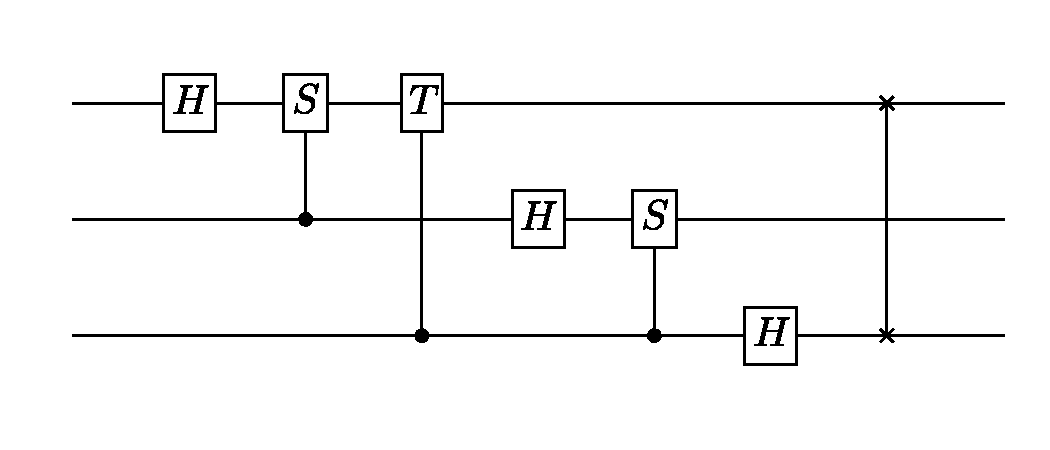
\includegraphics[scale=0.65]{images/fig1-circuitplot-qft}
\caption{The circuit diagram for a three-qubit quantum Fourier transform
generated by SymPy.}
\label{fig-circuitplot-qft}
\end{center}
\end{figure}
Lastly, the following example demonstrates creating a three-qubit quantum Fourier
transform, decomposing it into one- and two-qubit gates, and then generating a
circuit plot for the sequence of gates (see Figure~\ref{fig-circuitplot-qft}).
% This depends on matplotlib. We want to make sure the rest of the paper
% doesn't depend on it, so skip.
% no-doctest
\begin{verbatim}
>>> from sympy.physics.quantum.qft import QFT
>>> from sympy.physics.quantum.circuitplot import circuit_plot
>>> fourier = QFT(0,3).decompose()
>>> fourier
SWAP(0,2)*H(0)*C((0),S(1))*H(1)*C((0),T(2))*C((1),S(2))*H(2)
>>> c = circuit_plot(fourier, nqubits=3)
\end{verbatim}


\section{Architecture}
\label{sec:architecture}

Software architecture is of central importance in any large software
project because it establishes predictable patterns of usage and
development~\cite{Shaw1996}. This section describes the essential
structural components of SymPy, provides justifications for the design
decisions that have been made, and gives example
user-facing code as appropriate.

\subsection{The Core}
\label{sec:core}
A computer algebra system stores mathematical expressions as data structures.
For example, the mathematical expression $x + y$ is represented as a tree with
three nodes, $+$, $x$, and $y$, where $x$ and $y$ are ordered children of $+$.
As users manipulate mathematical expressions with traditional mathematical
syntax, the CAS manipulates the underlying data structures. Symbolic
computations such as integration, simplification, etc.\ are all functions that
consume and produce expression trees.

In SymPy every symbolic expression is an instance of the class
\texttt{Basic},\footnote{Some internal classes, such as those used in the
  polynomial submodule, do not follow this rule for efficiency reasons.} the
superclass of all SymPy types providing common methods to all SymPy
tree-elements, such as traversals. The children of a node in the tree are held
in the \texttt{args} attribute. A leaf node in the expression tree
has empty \texttt{args}.

For example, consider the expression $xy + 2$:
\begin{verbatim}
>>> x, y = symbols('x y')
>>> expr = x*y + 2
\end{verbatim}
By order of operations, the parent of the expression tree for \texttt{expr} is
an addition. It is of type \texttt{Add}. The child nodes of \texttt{expr} are
\texttt{2} and \texttt{x*y}.
\begin{verbatim}
>>> type(expr)
<class 'sympy.core.add.Add'>
>>> expr.args
(2, x*y)
\end{verbatim}

Descending further down into the expression tree yields the full expression. For
example, the next child node (given by \texttt{expr.args[0]}) is
\texttt{2}. Its class is \texttt{Integer}, and it has an empty \texttt{args}
tuple, indicating that it is a leaf node.
\begin{verbatim}
>>> expr.args[0]
2
>>> type(expr.args[0])
<class 'sympy.core.numbers.Integer'>
>>> expr.args[0].args
()
\end{verbatim}
Symbols or symbolic constants, like $e$ or $\pi$, are other examples of
leaf nodes.
\begin{verbatim}
>>> exp(1)
E
>>> exp(1).args
()
>>> x.args
()
\end{verbatim}

A useful way to view an expression tree is using the \texttt{srepr} function, which
returns a string representation of an expression as valid Python code\footnote{
\label{note:dotprint}
The \texttt{dotprint} function from the \texttt{sympy.printing.dot} submodule
prints output to dot format, which can be rendered with Graphviz to
visualize expression trees graphically.}
with all the nested class constructor calls to create the given expression.
\begin{verbatim}
>>> srepr(expr)
"Add(Mul(Symbol('x'), Symbol('y')), Integer(2))"
\end{verbatim}

Every SymPy expression satisfies a key identity invariant:
\begin{verbatim}
expr.func(*expr.args) == expr
\end{verbatim}
This means that expressions are
rebuildable from their \texttt{args}.\footnote{\texttt{expr.func} is used
instead of \texttt{type(expr)} to allow the function of an expression to be
distinct from its actual Python class. In most cases the two are the same.}
Note that in SymPy the \texttt{==} operator represents exact
structural equality, not mathematical equality. This allows testing if any two
expressions are equal to one another as expression trees. For example, even
though ${(x + 1)}^2$ and $x^2 + 2x + 1$ are equal mathematically, SymPy gives
\begin{verbatim}
>>> (x + 1)**2 == x**2 + 2*x + 1
False
\end{verbatim}
because they are different as expression trees (the former is a \verb|Pow|
object and the latter is an \verb|Add| object).

Another important property of SymPy expressions is that they are immutable.
This simplifies the design of SymPy, and enables expression interning. It also
enables expressions to be hashed, which allows expressions to be used as keys
in Python dictionaries, and is used to implement caching in SymPy.

Python allows classes to override mathematical operators. The Python
interpreter translates the above \texttt{x*y + 2} to, roughly,
\verb|(x.__mul__(y)).__add__(2)|. Both \texttt{x} and \texttt{y}, returned
from the \texttt{symbols} function, are \texttt{Symbol} instances. The
\texttt{2} in the expression is processed by Python as a literal, and is
stored as Python's built in \texttt{int} type. When \texttt{2} is passed to the
\verb|__add__| method of \texttt{Symbol}, it is converted to the SymPy type
\verb|Integer(2)| before being stored in the resulting expression tree. In
this way, SymPy expressions can be built in the natural way using Python
operators and numeric literals.

%% TODO: describe how assumptions are implemented

%%
%% Extensibility
\subsection{Extensibility}

While the core of SymPy is relatively small, it has been extended to a wide variety
of domains by a broad range of contributors.
This is due, in part, to the fact that the same language, Python,
is used both for the internal implementation and the external usage by users.
All of the extensibility capabilities available to
users are also utilized by SymPy itself. This eases the transition pathway from
SymPy user to SymPy developer.

The typical way to create a custom SymPy object is to subclass an existing
SymPy class, usually \texttt{Basic}, \texttt{Expr}, or \texttt{Function}. As
it was stated before, all SymPy classes used for expression trees should be
subclasses of the base class \texttt{Basic}. \texttt{Expr} is the
\texttt{Basic} subclass for mathematical objects that can be added and
multiplied together. The most commonly seen classes in SymPy are subclasses of
\texttt{Expr}, including \texttt{Add}, \texttt{Mul}, and \texttt{Symbol}.
Instances of \texttt{Expr} typically represent complex numbers, but may also
include other ``rings'', like matrix expressions. Not all SymPy classes are
subclasses of \texttt{Expr}. For instance, logic expressions, such as
\verb|And(x, y)|, are subclasses of \texttt{Basic} but not of
\texttt{Expr}.\footnote{See section~\ref{S-suppsec:Logic} of the supplementary
  material for more information on the
  \texttt{sympy.logic} submodule.}

The \texttt{Function} class is a subclass of \texttt{Expr} which makes it
easier to define mathematical functions called with arguments. This includes
named functions like $\sin(x)$ and $\log(x)$ as well as undefined functions
like $f(x)$. Subclasses of \texttt{Function} should define a
class method \texttt{eval}, which returns an evaluated value for the function
application (usually an instance of some other class, e.g., a \texttt{Number}),
or \texttt{None} if for the given arguments it should not be
automatically evaluated.

Many SymPy functions perform various evaluations down the expression tree.
Classes define their behavior in such functions by defining a relevant
\verb|_eval_|\texttt{\textit{*}} method. For instance, an object can indicate
to the \texttt{diff} function how to take the derivative of itself by defining
the \verb|_eval_derivative(self, x)| method, which may in turn call
\texttt{diff} on its \texttt{args}. (Subclasses of \texttt{Function} should
implement the \texttt{fdiff} method instead; it returns the derivative of the function
without considering the chain rule.) The most common
\verb|_eval_|\texttt{\textit{*}} methods relate to the assumptions:
\verb|_eval_is_|\texttt{\textit{assumption}} is used to deduce
\textit{assumption} on the object.

Listing~\ref{fig:gamma-example} presents an example of this extensibility. It
gives a stripped down version of the \texttt{gamma} function $\Gamma(x)$ from
SymPy. The methods defined allow it to evaluate itself on positive integer
arguments, define the real assumption, allow it to be rewritten in terms of
factorial (with \verb|gamma(x).rewrite(factorial)|), and allow it to be
differentiated. \texttt{self.func} is used throughout instead of referencing
\texttt{gamma} explicitly so that potential subclasses of \texttt{gamma} can
reuse the methods.

\lstset{
  basicstyle=\ttfamily,
}

\begin{lstlisting}[caption={A minimal implementation of \texttt{sympy.gamma}.},label=fig:gamma-example]
from sympy import Function, Integer, factorial, polygamma

class gamma(Function):
    @classmethod
    def eval(cls, arg):
        if isinstance(arg, Integer) and arg.is_positive:
            return factorial(arg - 1)

    def _eval_is_real(self):
        x = self.args[0]
        # noninteger means real and not integer
        if x.is_positive or x.is_noninteger:
            return True

    def _eval_rewrite_as_factorial(self, z):
        return factorial(z - 1)

    def fdiff(self, argindex=1):
        from sympy.core.function import ArgumentIndexError
        if argindex == 1:
            return self.func(self.args[0])*polygamma(0, self.args[0])
        else:
            raise ArgumentIndexError(self, argindex)
\end{lstlisting}
The gamma function implemented in SymPy has many more capabilities than the
above listing, such as evaluation at rational points and series expansion.


\subsection{Performance}
\label{sec:performance}

Due to being written in pure Python without the use of extension modules,
SymPy's performance characteristics are generally poorer than that of
its commercial competitors. For many applications,
the performance of SymPy, as measured by clock cycles, memory usage, and memory
layout, is sufficient.
However, the boundaries for when SymPy's pure Python strategy becomes
insufficient are when the user requires handling of very long expressions or many
small expressions. Where this boundray lies depends on the system at hand, but tends
to be within the range of $10^4$--$10^6$ symbols for modern computers.

For this reason, a new project called SymEngine~\cite{SymEngine} has been started.
The aim of this poject is to develop a library with better performance
characteristics for symbolic manipulation. SymEngine is a pure C++ library,
which allows it fine-grained control over the memory layout of expressions.
SymEngine has thin wrappers to other languages (Python, Ruby,
Julia, etc.). Its aim is to be the fastest symbolic manipulation library. Preliminary
benchmarks suggest that SymEngine performs as well as its commercial and
open source competitors.

The development version of SymPy has recently started to use SymEngine as an
optional backend, initially in \texttt{sympy.\allowbreak{}physics.\allowbreak{}mechanics} only.
Future work will involve
allowing more algorithms in SymPy to use SymEngine as a backend.


\section{Projects that Depend on SymPy}
\label{sec:other-proj}
There are several projects that depend on SymPy as a library for implementing
a part of their functionality. A selection of these projects are listed in
Table~\ref{projects-table}.

\begin{longtable}[htbc]{>{\raggedright}p{0.2\linewidth}p{0.74\linewidth}}
\caption{Selected projects that depend on SymPy.\label{projects-table}}\\
\toprule
\textbf{Project name} & \textbf{Description} \\
\midrule

\href{http://sympygamma.com/}{\textbf{SymPy Gamma}} & An open source
  analog of Wolfram|Alpha that uses SymPy~\cite{SymPyGamma}.  There is more
  information about SymPy Gamma in section~\ref{S-suppsec:sympy-gamma} of the
  supplementary material. \\

\href{http://cadabra.science/index.html}{\textbf{Cadabra}} &
  A CAS designed specifically for the resolution of problems
  encountered in field theory~\cite{Peeters2007cadabra}. \\

\href{https://github.com/cbm755/octsympy}{\textbf{GNU Octave Symbolic Package}} &
  An implementation of a symbolic toolbox for Octave using SymPy~\cite{OctSymPy}. \\

\href{https://github.com/jverzani/SymPy.jl}{\textbf{SymPy.jl}} &
  A Julia interface to SymPy, provided using PyCall~\cite{SymPy.jl}. \\

\href{https://mathics.github.io/}{\textbf{Mathics}} &
  A free, online CAS featuring Mathematica compatible
  syntax and functions~\cite{Mathics}. \\

\href{http://mathpix.com/}{\textbf{Mathpix}} & An iOS App that detects handwritten math as input and uses
  SymPy Gamma to evaluate the math input and generate the relevant
  steps to solve the problem~\cite{Mathpix}. \\

\href{http://openrave.org/docs/latest_stable/openravepy/ikfast/}{\textbf{IKFast}} &
  A robot kinematics compiler provided by
  \href{http://openrave.org/}{OpenRAVE}~\cite{diankov2010ikfast}. \\

\href{http://www.sagemath.org/}{\textbf{SageMath}} &
  A free open-source mathematics software system, which builds on top of many
  existing open-source packages, including SymPy~\cite{sagemath}. \\

\href{http://www.pydy.org/}{\textbf{PyDy}} & Multibody Dynamics with
  Python~\cite{gede2013constrained}. \\

\href{https://github.com/brombo/galgebra}{\textbf{galgebra}} &
  A Python package for geometric algebra (previously \texttt{sympy.galgebra})~\cite{galgebra}. \\

\href{http://yt-project.org/}{\textbf{yt}} & A Python package for
  analyzing and visualizing volumetric data~\cite{2011ApJS..192....9T}. \\

\href{http://sfepy.org/}{\textbf{SfePy}} &
  A Python package for solving partial
  differential equations (PDEs) in 1D, 2D, and 3D by the finite element (FE)
  method~\cite{Zienkiewicz2013finite,cimrman2014sfepy}. \\

\href{http://quameon.sourceforge.net/}{\textbf{Quameon}} & Quantum
  Monte Carlo in Python~\cite{quameon}. \\

\href{http://lcapy.elec.canterbury.ac.nz/}{\textbf{Lcapy}} &
  An experimental Python package for teaching linear circuit analysis~\cite{lcapy}. \\
\bottomrule
\end{longtable}


\section{Conclusion and Future Work}
\label{sec:conclusion}

SymPy is a robust computer algebra system that provides a wide spectrum of
features both in traditional computer algebra and in a plethora of scientific
disciplines. It can be used in a first-class way with other
Python projects, including the scientific Python stack.


SymPy supports a wide array of mathematical facilities. These include
functions for assuming and deducing common mathematical facts,
simplifying expressions, performing common calculus operations, manipulating polynomials, pretty printing
expressions, solving equations, and representing symbolic matrices. Other supported
facilities
include discrete math, concrete math, plotting, geometry, statistics,
sets, series, vectors, combinatorics, group theory, code
generation, tensors, Lie algebras, cryptography, and special functions.
SymPy has strong support for arbitrary precision numerics, backed by the
mpmath package. Additionally, SymPy contains submodules targeting certain specific physics domains,
such as classical mechanics and quantum mechanics.  This breadth of domains has
been engendered by a strong and vibrant user community.
Anecdotally, many of these users chose SymPy because of its ease of access.
SymPy is a dependency of many external projects across a wide
spectrum of domains.

SymPy expressions are immutable trees of Python objects. Unlike many other
CAS's, SymPy is designed to be used in an extensible way: both as an end-user
application and as a library. SymPy uses Python both as the internal language
and the user language. This permits users to access the same methods used
by the library itself in order to extend it for their needs.

% Future work:

Some of the planned future work for SymPy includes work on improving code
generation, improvements to the speed of SymPy using SymEngine, improving the
assumptions system, and improving the solvers submodule.

% TODO: Maybe one sentence for each item

% Feel free to add stuff here.


\phantomsection
\bibliography{paper}

\end{document}
